\documentclass[conference]{IEEEtran}
\IEEEoverridecommandlockouts
% The preceding line is only needed to identify funding in the first footnote. If that is unneeded, please comment it out.
\usepackage{url}


\usepackage{ragged2e, tabularx, makecell, booktabs}
\usepackage{multirow}
\usepackage{cite}
\usepackage{amsmath,amssymb,amsfonts}
\usepackage{algorithmic}
\usepackage{graphicx}
\usepackage{textcomp}
\usepackage{xcolor}
\usepackage{hyperref}
\usepackage{fontawesome5}
\def\BibTeX{{\rm B\kern-.05em{\sc i\kern-.025em b}\kern-.08em
    T\kern-.1667em\lower.7ex\hbox{E}\kern-.125emX}}
\begin{document}

\title{A Monte Carlo Tree Search for the
Optimisation of Flight Connections
}

\author{\IEEEauthorblockN{Arnaud Da Silva\IEEEauthorrefmark{1}, Ahmed Kheiri\IEEEauthorrefmark{1}}
\IEEEauthorblockA{\IEEEauthorrefmark{1}Lancaster University, Department of Management Science, Lancaster LA1 4YX, UK
\\ \{a.dasilva, a.kheiri\}@lancaster.ac.uk}}


\maketitle

\begin{abstract}
In 2017, Kiwi.com proposed the Travelling Salesman Problem 2.0. Despite some similarities with the classic Travelling Salesman Problem (TSP), the problem is more complex. It can be characterised as an asymmetric, time-constrained and generalised TSP. Moreover, infeasibility further complicates the challenge, as no flights may be available between certain airports on specific days. Exact methods often fail in solving these $\mathcal{NP}$-Hard problems. Therefore, alternative approaches, such as heuristics, are typically favoured. A Monte Carlo Tree Search (MCTS) is implemented to tackle Kiwi's problem, an algorithm traditionally used in board games but adapted here for air travel optimisation. The MCTS has been chosen for its proven effectiveness in handling complex and high-dimensional search spaces.

\end{abstract}

\begin{IEEEkeywords}
Optimisation, Travelling Salesman Problem, Monte Carlo Tree Search, Heuristic Design.
\end{IEEEkeywords}

\section{Introduction}

The number of flight connections continues to grow each year \cite{statista_flights_year}, with over 38 million flights scheduled in 2023. This increasing volume poses a significant challenge for travellers trying to find the best and cheapest flight connections for their specific journeys, particularly when multiple cities are involved. As a result, travel agencies have implemented online trip planner algorithms to help travellers find flights that meet their requirements. Examples of such platforms include Google Flights, OpenFlights.org, Skyscanner, Kayak, and Kiwi.com. 
%
These agencies have introduced various challenges to develop more powerful trip planner algorithms. For example, as noted in \cite{reinforcement_learning_yaro}, OpenFlights.org launched the Air Travelling Salesman Project. Similarly, in 2017, Kiwi.com initiated the Travelling Salesman Challenge, which led to the development of their current algorithm. In 2018, Kiwi.com introduced a new challenge, the Travelling Salesman Problem 2.0, which is the focus of this study. Despite the large number of participants in these challenges, there is limited literature on the methods employed. The winning team used a breadth-first search (BFS) algorithm \cite{tsp2_award}, while other participants applied heuristics such as simulated annealing, genetic algorithms, and reinforcement learning. Only two papers have been published on these approaches \cite{reinforcement_learning_yaro,local_search_yaro}, focusing on local search and reinforcement learning. This scarcity of research inspired our decision to implement a novel solution using Monte Carlo Tree Search (MCTS) to tackle the problem. 

The problem at hand is a variant of the well-known Travelling Salesman Problem (TSP). It can be described as a generalised, asymmetric, and time-dependent TSP. A traveller must visit a set of areas, one per day, starting from a given airport, with various flight connections available between these airports on different days. The objective is to determine the cheapest flight route that allows the traveller to return to the starting location. Due to the large number of possible routes, solving this problem by exhaustively exploring every potential solution is infeasible. Therefore, a heuristic approach is employed. 

\section{Problem description}

Kiwi's traveller plans to visit \(N\) different areas over \(N\) days. Let \(A\) denote the set of areas the traveller intends to visit:  
$A = \{A_1, A_2, \ldots, A_N\}$, where each \(A_j\) is a set of airports within area \(j\), represented as:  $A_j = \{a_{j,1}, a_{j,2}, \ldots, a_{j,k_j}\}$. Here, \(a_{j,k_j}\) represents the airports in area \(j\), and \(k_j\) is the number of airports in area \(j\). 
%
The traveller must visit one area per day. They have to leave each area to visit a new one by departing from the same airport they arrived at. The journey starts from a known airport, and the traveller must complete the trip by returning to the starting area, though not necessarily to the starting airport. 
%
There are flight connections between different airports, with varying prices depending on the day of travel. Let \(c^{d}_{ij}\) represent the cost to travel from city \(i\) to city \(j\) on day \(d\). It is not necessarily true that \(c^{d}_{ij} = c^{d}_{ji}\), nor that \(c^{d_1}_{ij} = c^{d_2}_{ij}\) if \(d_1 \neq d_2\). Moreover, \(\exists  d\) such that \(c^{d}_{ij} = \infty\), meaning there is no flight connection between city \(i\) and city \(j\) on day \(d\). 
%
The aim of the problem is to find the cheapest route for the traveller's journey. 
%
The problem has not been mathematically defined in previous research. Therefore, we can formulate the problem as follows:

\begin{itemize}
    \item $\mathcal{A} = \{1, 2, \ldots, N\}$: Set of areas.
    \item $A_j = \{a_{j,1}, a_{j,2}, \ldots, a_{j,k_j}\}$: Set of airports in area $j \in \mathcal{A}$.
    \item $\mathcal{D} = \{1, 2, \ldots, N\}$: Set of days.
    \item $U_d \subseteq \mathcal{A}$: Set of areas that have not been visited by the end of day $d$.
\end{itemize}

\subsection*{Parameters and Variables}
\begin{itemize}
    \item $c_{ij}^d$: Cost to travel from airport $i$ to airport $j$ on day $d \in \mathcal{D}$.
    \item $x_{ij}^d$: Binary variable, equal to 1 if the traveller flies from airport $i$ to airport $j$ on day $d$, and 0 otherwise.
    \item $v_j^d$: Binary variable, equal to 1 if area $j$ is visited on day $d$, and 0 otherwise.
\end{itemize}

\subsection*{Objective Function}
The goal is to minimise the total travel cost of the journey:
\begin{align}
\min \Bigg( &\sum_{d=2}^{N-1} \sum_{i \in \bigcup_{k=2}^{N-1} A_k} \sum_{j \in \bigcup_{k=3}^{N} A_k} c_{ij}^d x_{ij}^d \notag \\
           &+ \sum_{j \in A_1} c_{S_0,j}^1 x_{S_0,j}^1 + \sum_{i \in A_N} \sum_{j \in A_1} c_{ij}^N x_{ij}^N \Bigg)
\end{align}

\subsection*{Constraints}
\begin{itemize}
    \item Starting from the known starting airport \(S_{0}\) and taking an existing flight connection:
          \[
          \sum_{j \in A_1} x_{S_0,j}^1 = 1 \quad \text{and} \quad \forall d \in \mathcal{D}, c_{S_0,j}^{d} \in \mathbb{R}^{+*}
          \]

    \item Visit exactly one airport in each area each day:
          \[
          \sum_{i \in A_d} \sum_{j \in A_{d+1}} x_{ij}^d = 1 \quad \forall d \in \{1, 2, \ldots, N-1\}
          \]

    \item Ensure the traveller departs from the same airport they arrived at the previous day:
          \[
          \sum_{k \in A_d} x_{ik}^d = \sum_{k \in A_{d-1}} x_{ki}^{d-1} \quad \forall i \in \bigcup_{j=1}^N A_j, \forall d \in \{2, 3, \ldots, N\}
          \]

    \item Return to an airport in the starting area on the final day with an existing flight connection:
          \[
          \sum_{i \in A_N} \sum_{j \in A_1} x_{ij}^N = 1 \quad \text{and} \quad \forall (i,j) \in A_N \times A_1, c_{ij}^{N} \in \mathbb{R}^{+*}
          \]

    \item Ensure each area is visited exactly once:
          \[
          \sum_{d \in \mathcal{D}} v_j^d = 1 \quad \forall j \in \mathcal{A}
          \]

    \item Update the unvisited list:
          \[
          v_j^d = 1 \implies j \notin U_d \quad \forall j \in \mathcal{A}, \forall d \in \mathcal{D}
          \]

    \item Ensure a flight on day \(d\) between airports \(i\) and \(j\) exists only if the cost exists and area \(j\) is unvisited on day \(d\):
          \[
          x_{ij}^d \leq c_{ij}^d \cdot v_j^d \quad \forall i, j \in \left( \bigcup_{j=1}^N A_j \right)^2, \forall d \in \mathcal{D}
          \]
          \[
          x_{ij}^d \leq v_j^d \quad \forall j \in \bigcup_{j=1}^N A_j, \forall d \in \mathcal{D}
          \]

    \item Binary variable constraints:
          \[
          x_{ij}^d \in \{0, 1\} \quad \forall (i, j) \in \left( \bigcup_{j=1}^N A_j \right)^2, \forall d \in \mathcal{D}
          \]
          \[
          v_j^d \in \{0, 1\} \quad \forall j \in \mathcal{A}, \forall d \in \mathcal{D}
          \]
\end{itemize}

%\subsection{Test Instances}

%We are given a set of 14 instances \( I_{n} = \{I_1, I_2, \ldots, I_{13}, I_{14}\} \). For each instance \( I_i \), we know the available flight connections between two airports on specific days and their associated costs. In some instances, flights may be available on day 0, meaning these connections exist for every day of the journey at the same price. Moreover, there may be multiple flights between the same airports on a specific day, but with varying prices. In such cases, we consider only the most relevant connections, i.e., the flight connection with the lowest fare. 


\section{Methodology}

\subsection{Selection Policy}

The selection phase of the Monte Carlo Tree Search (MCTS) algorithm uses the \textit{Upper Confidence Bound (UCB)} strategy to balance exploration and exploitation. This involves selecting the node that minimises the UCB or the UCB1-Tuned score, calculated as: $UCB = \overline{X}_i + C_p \sqrt{\frac{2 \ln N}{n_i}}$

\begin{equation}
    UCB1T = \overline{X}_i + \sqrt{\frac{\ln N}{n_i} \min\left(\frac{1}{4}, \mathrm{Var}(X_i) + \sqrt{\frac{2 \ln N}{n_i}}\right)}
    \nonumber
\end{equation}

Where:
\begin{itemize}
    \item \( \overline{X}_i \): The average reward of node \( i \).
    \item \( N \): The total number of visits to the root node.
    \item \( n_i \): The number of visits to node \( i \).
    \item \( C_p \): Exploration parameter.
    \item \( \mathrm{Var}(X_i) \): The variance of the rewards at node \( i \), representing the variability of the rewards.
\end{itemize}

The UCB balances exploration with the coefficient $C_p$, where empirically $C_p = \sqrt{2}$. The term \( C_p \sqrt{\frac{2 \ln N}{n_i}} \) adds a confidence interval to the average reward, which encourages exploring less-visited nodes when $C_p > 0$. When $C_p = 0$, the tree search explores less but exploits more of the known part that appears promising for the problem in the tree.

The UCB1-Tuned balances its exploration with \( \min\left(\frac{1}{4}, \mathrm{Var}(X_i) + \sqrt{\frac{2 \ln N}{n_i}}\right) \), making UCB1-Tuned more adaptable to environments with varying reward distributions. The $C_p$ coefficient can also be considered in UCB1-Tuned's formula. Hence, in stochastic environments, UCB1-Tuned is more likely to exhibit better overall performance.

\subsection{Simulation Policy}

When a simulation is run from a given node in the tree, the goal is to find a feasible combination of airports that could be a solution to our problem. Three simulation policies have been implemented and are used to select the actions needed to reach a leaf node in the tree:

\begin{itemize}
    \item \textbf{Random policy}: This policy selects a random action from the set of available actions, introducing variability and exploration in the simulation process.
    \item \textbf{Greedy policy}: This policy selects the action that corresponds to the cheapest available flight connection, thus prioritising cost minimisation at each step.
    \item \textbf{Tolerance policy} (with coefficient $c$): This policy selects an action randomly from a subset of actions that are within a certain tolerance level $c$ of the minimum cost action. This policy introduces a more balanced approach than the random and greedy policies.
\end{itemize}

\subsection{Expansion Policy}

When expanding a node, it is theoretically possible to expand all available child nodes. However, in practice, this can be computationally expensive and time-consuming, particularly in problems with a large number of possible actions. To address this, heuristic approaches often involve compromises that enhance the efficiency of the search process by selectively expanding certain nodes rather than all possible ones.

\begin{itemize}
    \item \textbf{Top-K policy}: This policy expands the nodes corresponding to the cheapest flight connections available. It sorts all possible actions based on their associated costs and selects the top \(k\) actions with the lowest costs, where \(k\) is regulated by the allowed number of children \(N_c\).
    \item \textbf{Ratio policy}: This policy takes a more balanced approach by combining the selection of the best actions with a degree of randomness. First, it calculates the number of top actions to select based on a predefined ratio, \(c \in [0,1]\), which reflects the proportion of Top-K actions within the allowed \(N_c\). After selecting these best actions, the policy randomly selects \((1-c) \times N_c\) actions from the remaining pool to reach the desired number of children.
\end{itemize}

A $\mathcal{MCTS}$ function can be defined. The function parameters include $S_p(C_p)$ for the selection policy, $E_p(c)$ for the expansion policy, $R_p$ for the rollout policy, and \(N_c\), defining the maximum number of children expanded per node.

\subsection{Parallelisation}

In computer science, parallelisation is a technique that divides a number of tasks into sub-tasks that can be independently and simultaneously run on multiple cores of a computer. Due to the nature of MCTS and its four phases, this algorithm is a good candidate for parallelisation. For instance, after selecting a node to explore, rather than conducting a single simulation based on one simulation policy, you can either run simulations using multiple different simulation policies and select the best outcome, or perform multiple simulations using the same policy (if it is stochastic). This is known as leaf parallelisation \cite{different_selection_policies}.

\section{Computational Results}


The results presented in this section were generated using an Intel i7-10700 CPU with 8 cores at 3.30 GHz, and 16 GB of RAM. We utilised Python 3.10 within VS Code (version 1.92.2). For further details, please refer to \href{https://github.com/adasilva33/DASA_Kiwi_TSP_Challenge_2}{\faGithub\ GitHub} and \href{https://github.com/ahmedkheiri//DASA_Kiwi_TSP_Challenge_2}{\faGithub\ GitHub}. 
Simulations for each considered instance were conducted, testing various parameter combinations in the grid search defined in Table \ref{table:Grid search}. One challenge encountered was the computational budget when using Python. As a result, the size of the grid search for the more complex instances was reduced, as shown in Table \ref{table:Grid search}.

\begin{table}[h]
    \centering
    \caption{Grid search}
    \resizebox{.4\textwidth}{!}{ % Resize the table to fit the text width
        \begin{tabular}{c|c|c}
            \cmidrule(r){2-3}
                                        & ($I_1,\ldots,I_6$)        & ($I_7, I_8$)     \\
            \midrule
            \textit{selection\_policy}  & top\_k, ratio\_k          & top\_k, ratio\_k \\
            \textit{simulation\_policy} & random, greedy, tolerance & greedy           \\
            \textit{selection\_policy}  & UCB, UCB1T                & UCB              \\
            \textit{C\_p}               & 0, 1.4, 2.8               & 1.4              \\
            \textit{N\_c}               & 5, 10, 15                 & 10               \\
            \textit{Ratio c}            & 0, .3, .5, .8, 1          & .5               \\
            \textit{N° simulations}     & 10                        & 10               \\
            \bottomrule
        \end{tabular}
    }
    \label{table:Grid search}
\end{table}

After running the simulations with the grid search parameters defined in Table \ref{table:Grid search}, we compared our results with the best known solutions, as presented in Table \ref{table:Best result vs state of the art} \cite{reinforcement_learning_yaro}. Note that only a subset of problem instances was considered due to the computational complexity and time constraints associated with evaluating all possible configurations for larger instances. 

\begin{table}[h]
    \centering
        \caption{Best results vs State of the art. Solutions were found for instances $I_1$, $I_2$, $I_3$, $I_4$, $I_7$, and $I_8$}

    \resizebox{.4\textwidth}{!}{ % Resize the table to fit the text width
        \begin{tabular}{|>{\centering\arraybackslash}p{1cm}
            >{\centering\arraybackslash}p{1cm}
            >{\centering\arraybackslash}p{1cm}
            >{\centering\arraybackslash}p{1cm}
            >{\centering\arraybackslash}p{1cm}
            >{\centering\arraybackslash}p{1cm} |}
            \toprule
            Instance & Best known & Best found    & Gap (\%) & Mean & Std   \\
            \midrule
            $I_1$    & 1396       & \textbf{1396} & 0        & 1396    & 0     \\
            $I_2$    & 1498       & \textbf{1498} & 0        & 1498    & 0     \\
            $I_3$    & 7672       & \textbf{7672} & 0        & 7672    & 0     \\
            $I_4$    & 13952      & 15361         & 10.1     & 15361     & 0 \\
            $I_5$    & 690        & -             & -        &  -    & -     \\
            $I_6$    & 2159       & -             & -        & -     & -     \\
            $I_7$    & 30937      & 31924         & 3.19     & 30937    & 0     \\
            $I_8$    & 4052       & \textbf{4037} & -0.52    & 4052    & 0     \\
            \bottomrule
        \end{tabular}
    }
    \label{table:Best result vs state of the art}
\end{table}

For instances $I_1$, $I_2$, and $I_3$, solutions were found and the various simulations were carried out successfully. Consequently, we investigated the influence of the parameters on the $\mathcal{MCTS}$ function and the final solution. However, for instance $I_4$, only a few parameterisations of the $\mathcal{MCTS}$ algorithm were successful in finding a solution. Specifically, the UCB1T selection policy combined with the tolerance or random simulation policies resulted in trees that were too large to find solutions within a reasonable time frame.

\subsubsection*{Analysis on $C_p$}

\begin{figure}[!ht]
    \centering
    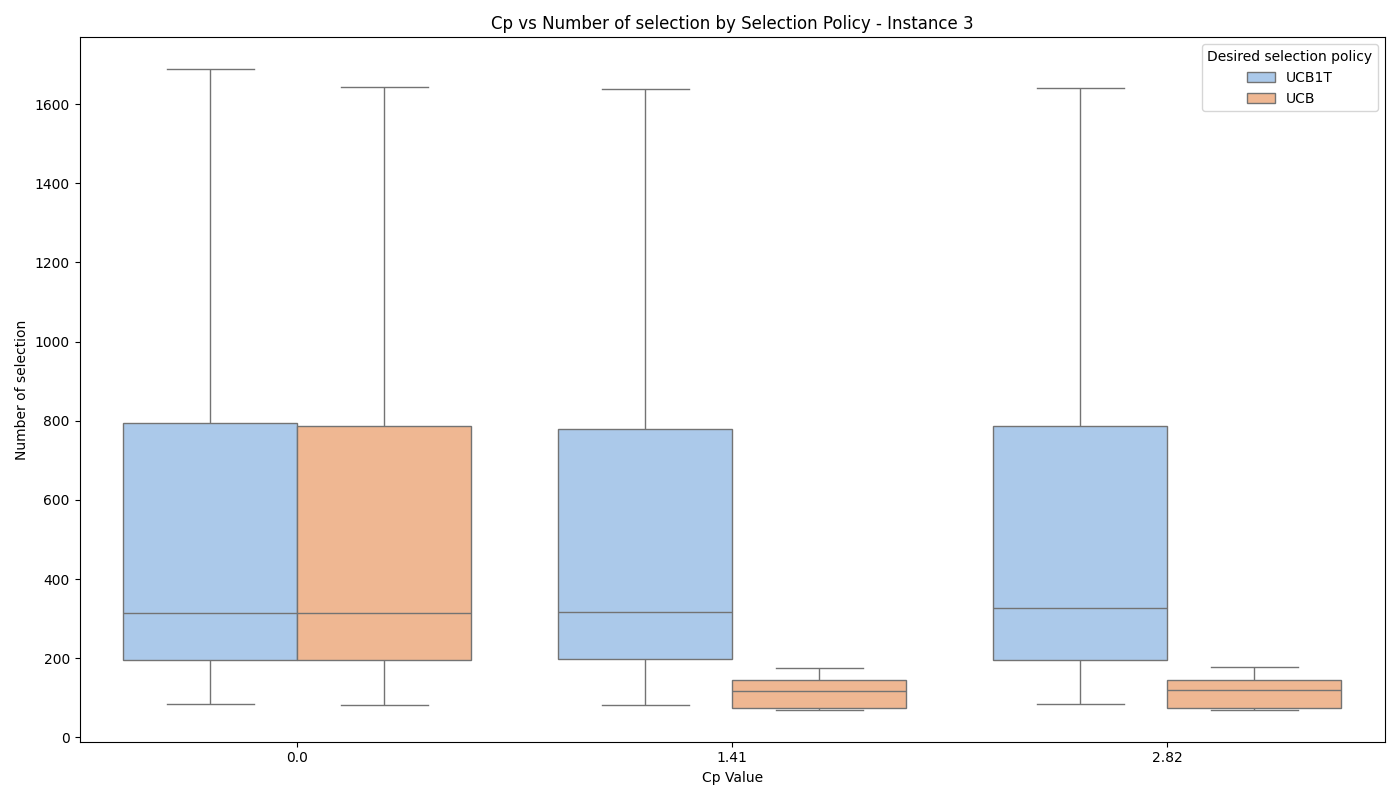
\includegraphics[width=.4\textwidth]{Figures/3 - cp_vs_selection.png}
    \caption{Effect of \(C_p\) on the Number of Selections}
    \label{fig:cp_vs_selection_3}
\end{figure}

Figure \ref{fig:cp_vs_selection_3} presents box plots illustrating the relationship between the exploration constant \(C_p\) and the number of selection phases under the UCB and UCB1T selection policies:

\begin{itemize}
    \item \textbf{\(C_p = 0\) leads to identical performance:}
          When \(C_p = 0\), the UCB and UCB1T selection policies are equivalent, resulting in identical decision-making during MCTS.
    \item \textbf{Higher \(C_p\) values lead to faster convergence for UCB:}
          As \(C_p\) increases from 0.0 to 2.82, the median number of selection phases under the UCB policy decreases.
    \item \textbf{UCB1T encourages more exploration:}
          UCB1T consistently results in a higher number of selection phases compared to UCB, particularly at higher \(C_p\) values. This aligns with UCB1T's design to promote broader exploration before converging.
\end{itemize}

While UCB1T may require more time to converge, it generally explores the search tree more effectively, leading to better overall performance. One can notice that $C_p$'s correlation with the UCB1T selection policy for $I_3$ is low.

\subsubsection*{Analysis of Expansion Ratio $c$}

When comparing the relationship between the expansion ratio (the proportion of expanded child nodes that have the cheapest flight connection among the chosen number of children) and the time required to find a solution for the UCB and UCB1T policies, several conclusions can be drawn:

\begin{itemize}
    \item \textbf{UCB finds solutions faster than UCB1T:}
          Across all expansion ratio values, the UCB policy consistently finds solutions more quickly than UCB1T. This suggests that UCB, being less aggressive in exploration, converges on solutions faster.

    \item \textbf{Higher ratios lead to faster convergence:}
          For both policies, the time to find a solution generally decreases as the expansion ratio increases. This indicates a more efficient search process when expanded nodes are less randomly chosen from the set of available actions. However, for more complex instances, maintaining a ratio \( r \in [0.3, 0.7] \) is crucial to avoid getting stuck in potential leaf nodes.
\end{itemize}

Finally, the UCB policy exhibits a stronger correlation with the expansion ratio compared to UCB1T, as shown in Figure \ref{fig:ratio_vs_cost_3}. Despite this correlation, UCB's overall performance is inferior to that of UCB1T. This is because UCB relies more heavily on exploitation, whereas UCB1T, though slower to converge, achieves better results by balancing exploration and exploitation more effectively.

\begin{figure}[!ht]
    \centering
    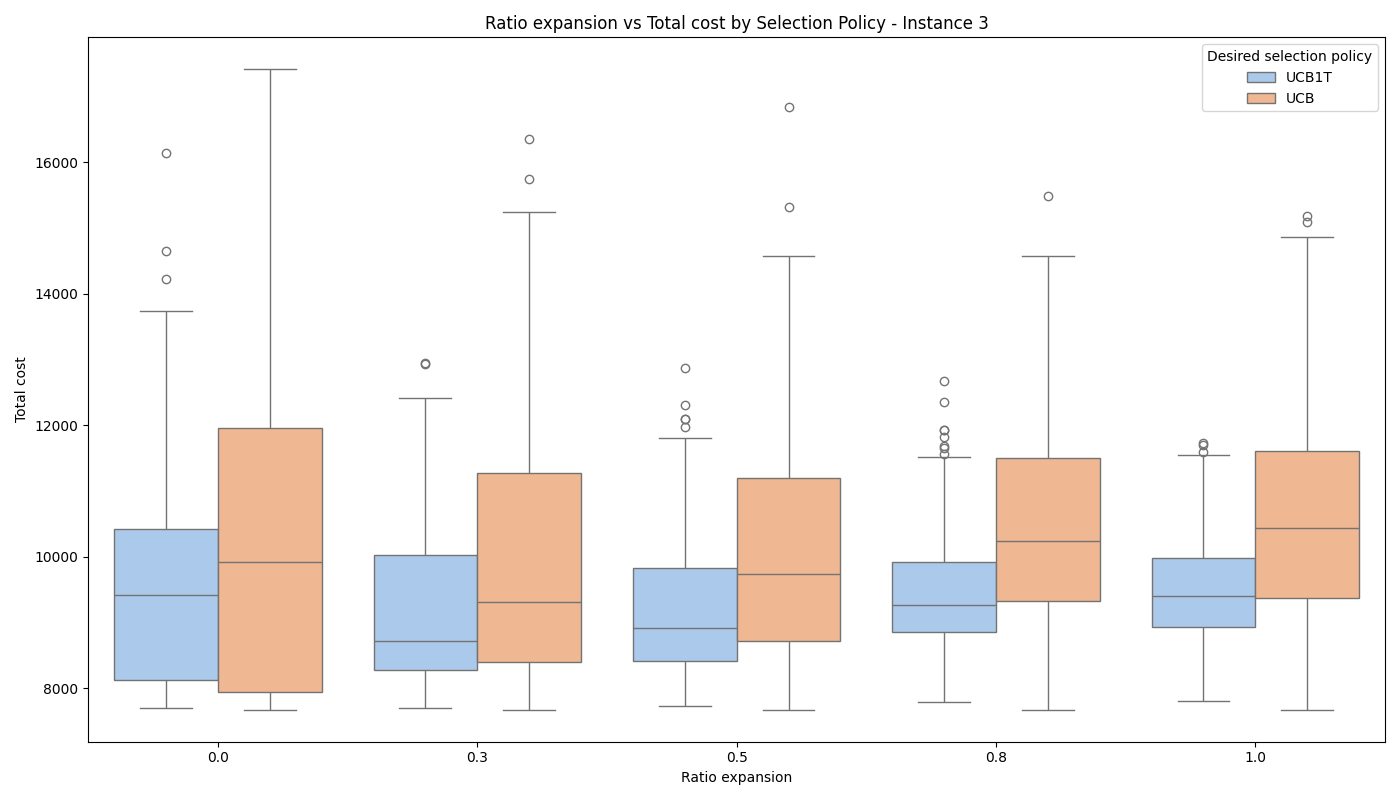
\includegraphics[width=.4\textwidth]{Figures/3 - ratio_vs_cost.png}
    \caption{Expansion ratio vs Total cost}
    \label{fig:ratio_vs_cost_3}
\end{figure}

\subsubsection*{Analysis of Simulation Performances}

\begin{figure}[!ht]
    \centering
    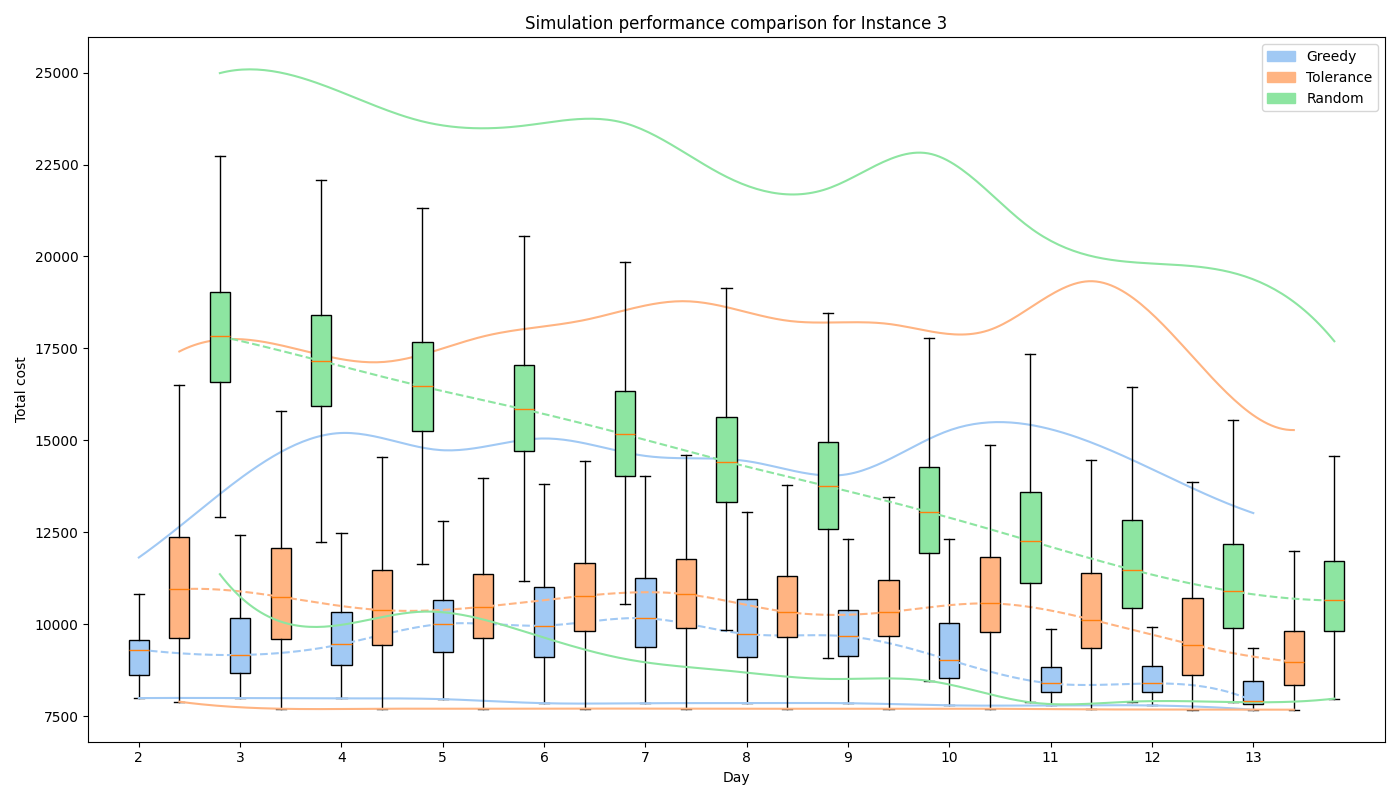
\includegraphics[width=.4\textwidth]{Figures/3 - Simulation performance.png}
    \caption{Simulation performance for Instance 3}
    \label{fig:sim_perf_3}
\end{figure}

Figure \ref{fig:sim_perf_3} presents box plots for the different simulation policies applied to Instance 3. For each day, the distribution of the simulated outcomes is plotted according to the simulation policy used. Coloured curves indicate the minimum and maximum values of these distributions, while dashed lines represent the medians.

In Figure \ref{fig:sim_perf_3}, the greedy simulation policy demonstrates superior performance, as evidenced by lower minimum, maximum, and median values of the simulation outcomes across all days. The pronounced convergence of the random policy reflects the inherent randomness of this approach. Additionally, for the greedy and tolerance policies, the minimum value is nearly reached by the second or third day of simulation. This suggests that a well-calibrated set of parameters for the $\mathcal{MCTS}$ algorithm should ideally converge towards the minimum cost observed during the simulations. If the algorithm does not achieve this, it indicates that the $\mathcal{MCTS}$ parameterisation may be suboptimal. 
Figure \ref{fig:sim_perf_vs_c_4} illustrates the distributions of simulated outcomes for a misparameterised $\mathcal{MCTS}$ instance ($I_4$). 

In Figure \ref{fig:sim_perf_vs_c_3}, the median distributions for different scenarios are plotted. The analysis reveals that values of $c$ too close to 1 do not, on average, converge to the minimum-cost solution. In contrast, lower values of $c$ tend to guide the tree search more effectively during the first days of simulations. This is crucial because it helps avoid excessive expansion of the search tree, which can lead to inefficient and time-consuming MCTS processes.

\begin{figure}[!ht]
    \centering
    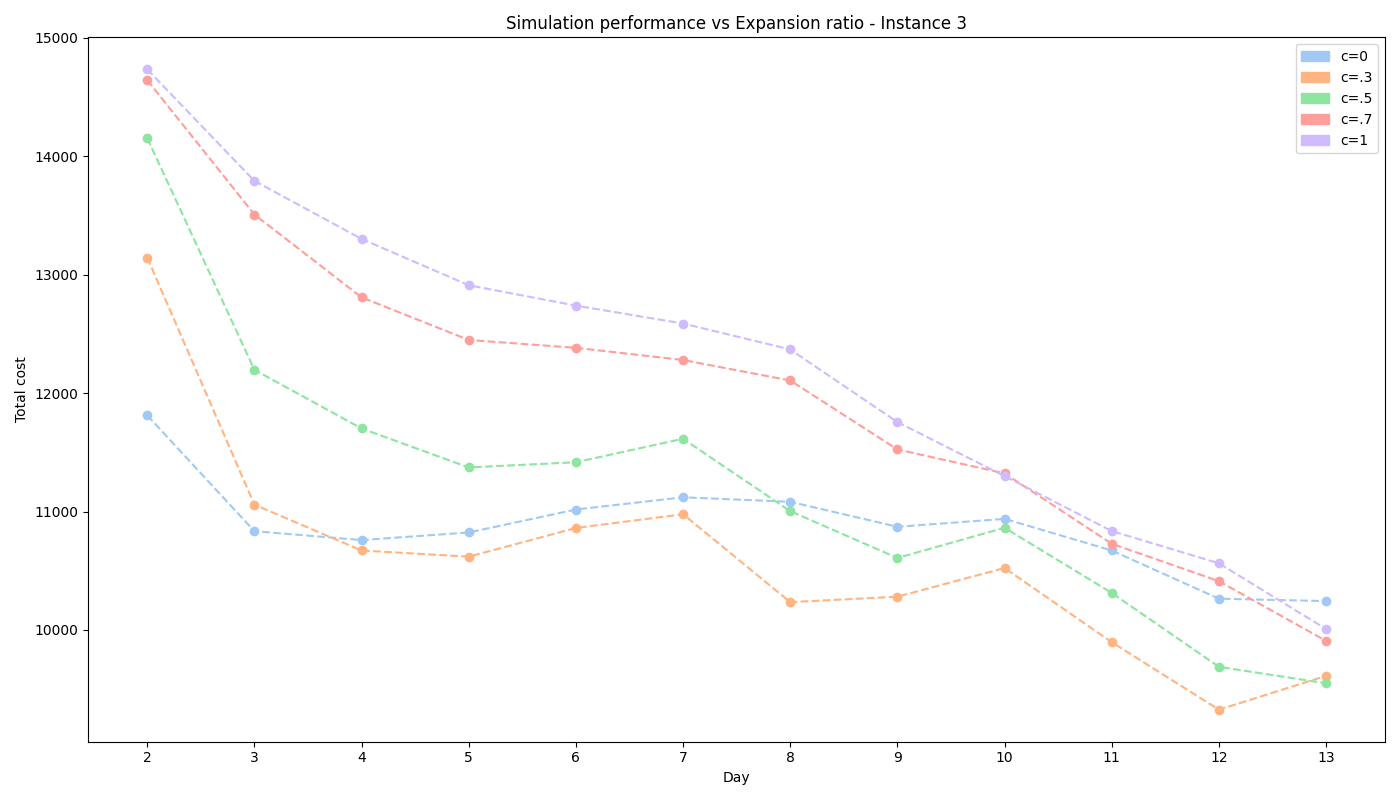
\includegraphics[width=.4\textwidth]{Figures/3 - Simulation performance vs Expansion ratio.png}
    \caption{Simulation performance vs Expansion Ratio - Instance 3}
    \label{fig:sim_perf_vs_c_3}
\end{figure}

These conclusions apply to smaller instances. However, for instance $I_4$, as shown in Figure \ref{fig:sim_perf_vs_c_4}, having $c=0$ with a greedy selection policy proves inefficient. The search tree diverges from the minimum simulated cost, resulting in the tree search failing to find a solution within 10 minutes. Based on the median comparison, $c=1$ emerges as a more optimal parameter for guiding the tree search in this case.

\begin{figure}[!ht]
    \centering
    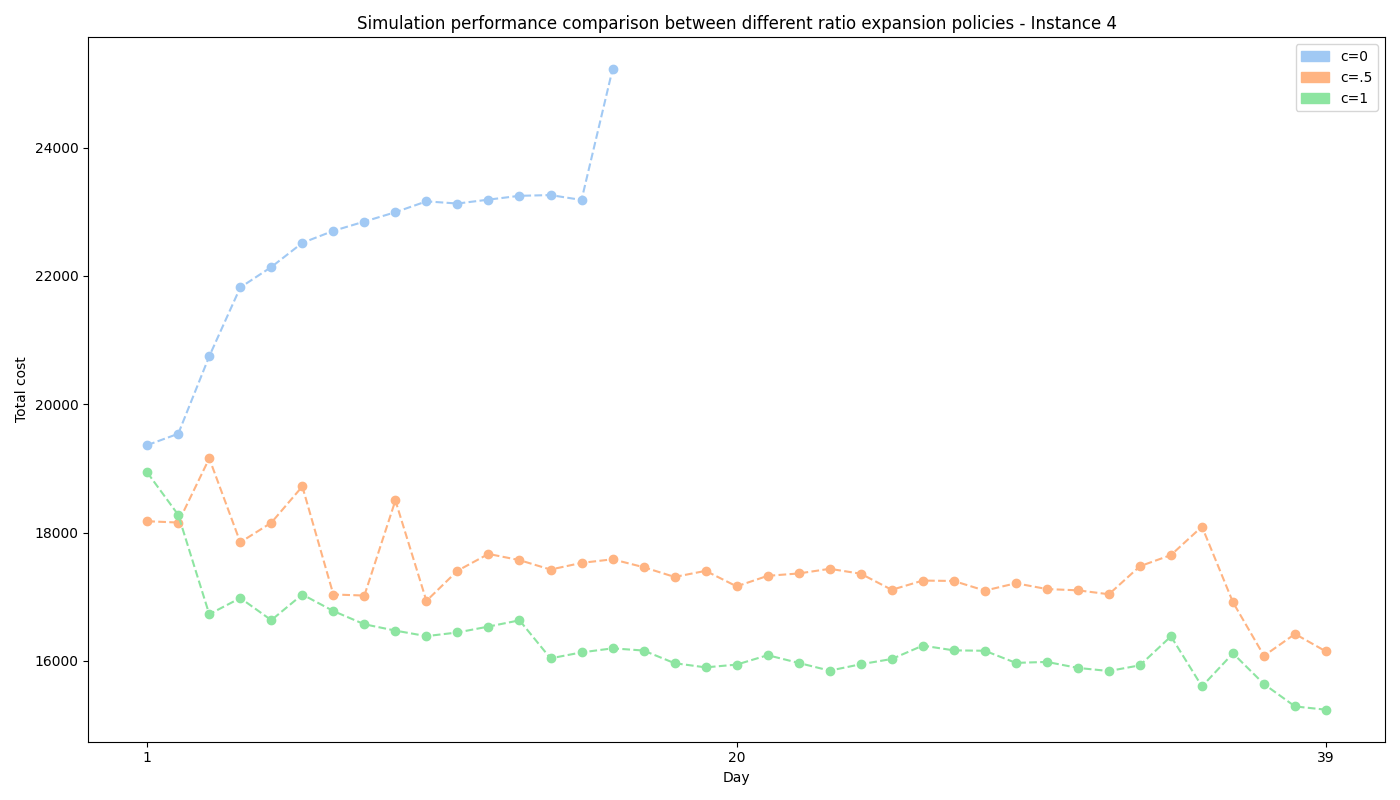
\includegraphics[width=.4\textwidth]{Figures/4 - Simulation performance vs Expansion ratio.png}
    \caption{Simulation performance vs Expansion Ratio - Instance 4}
    \label{fig:sim_perf_vs_c_4}
\end{figure}

The MCTS function struggled to effectively search the tree for instances $I_5$ and $I_6$ using grid search, as nodes simulated under random or tolerance policies that reached final states did not facilitate further tree expansion. Instances $I_7$ and $I_8$ were solved using a UCB selection policy with \(C_p = 1.41\) and \(N_c = 5\) under the top\_k expansion policy. For $I_7$, the solution found was higher by 3.19\% compared to the state of the art. In contrast, for $I_8$, a new state-of-the-art solution was achieved, improving the best known solution by 0.52\%.

\subsubsection*{Parallelisation}

In our implementation for instance $I_4$, we parallelised the MCTS across five cores. The parameters were selected to illustrate the effects of parallelisation in a stochastic environment. The parallelisation was applied during the simulation phase of the MCTS, with the minimum outcome from the five parallel simulations being chosen as the final result. In Figure \ref{fig:sim_perf_parral_4}, the distribution of outcomes from using five cores for parallelisation shows better performance compared to the non-parallelised approach. This confirms that parallelisation enhances the effectiveness of the MCTS, particularly in the initial days of the tree search.

\begin{figure}[!ht]
    \centering
    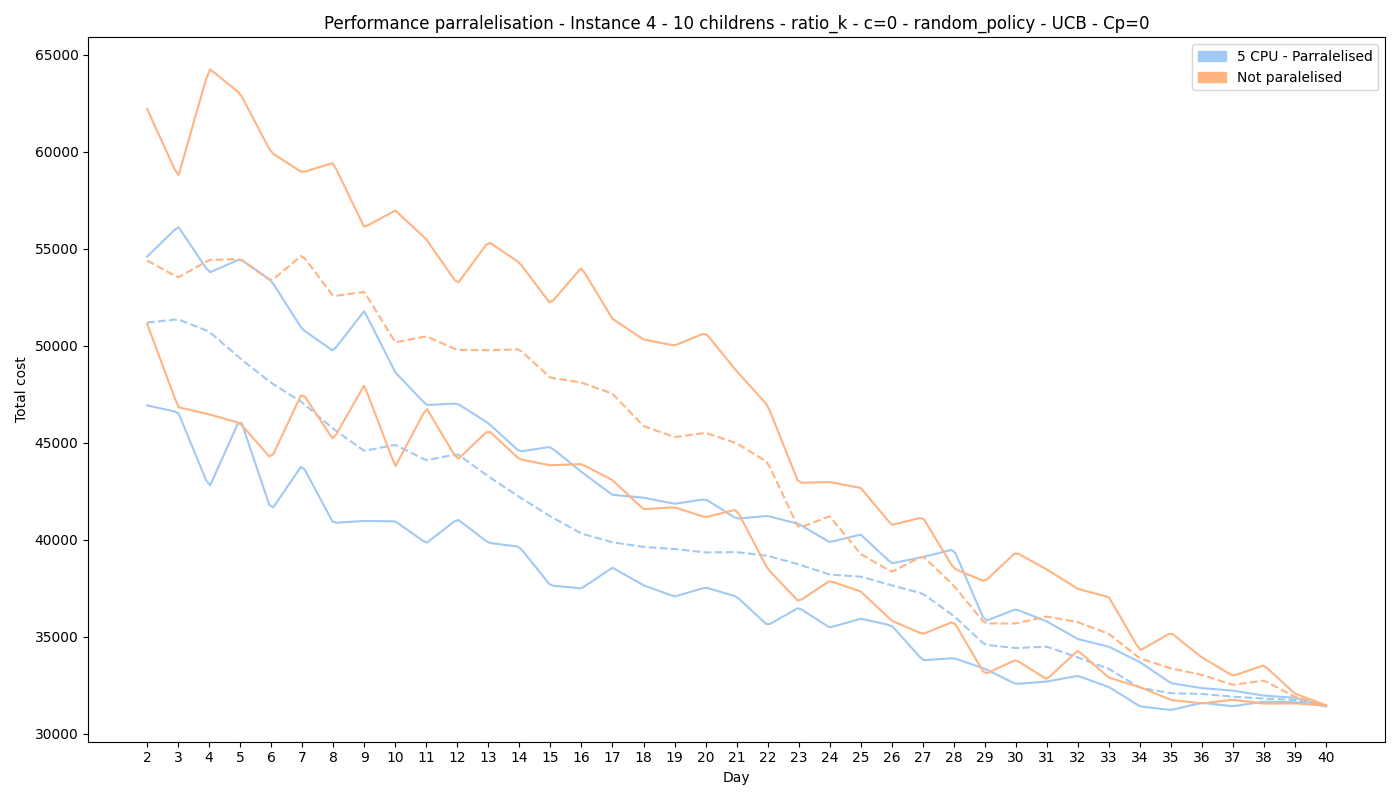
\includegraphics[width=.4\textwidth]{Figures/4 - Paralelised vs 5 CPU paralelised.png}
    \caption{Comparison of the distributions for the simulated outcomes without parallelisation and with 5 cores - Instance 4}
    \label{fig:sim_perf_parral_4}
\end{figure}


The comparative analysis of five-core and ten-core parallelisations of MCTS, evaluated using Mann-Whitney and Kolmogorov-Smirnov tests as shown in Figure \ref{fig:Stats test 5 VS 10 Parall}, revealed no statistically significant improvements at the 5\% level. As discussed in \cite{different_selection_policies}, excessive modifications to the MCTS can sometimes lead to undesirable behaviour.

\begin{figure}[!ht]
    \centering
    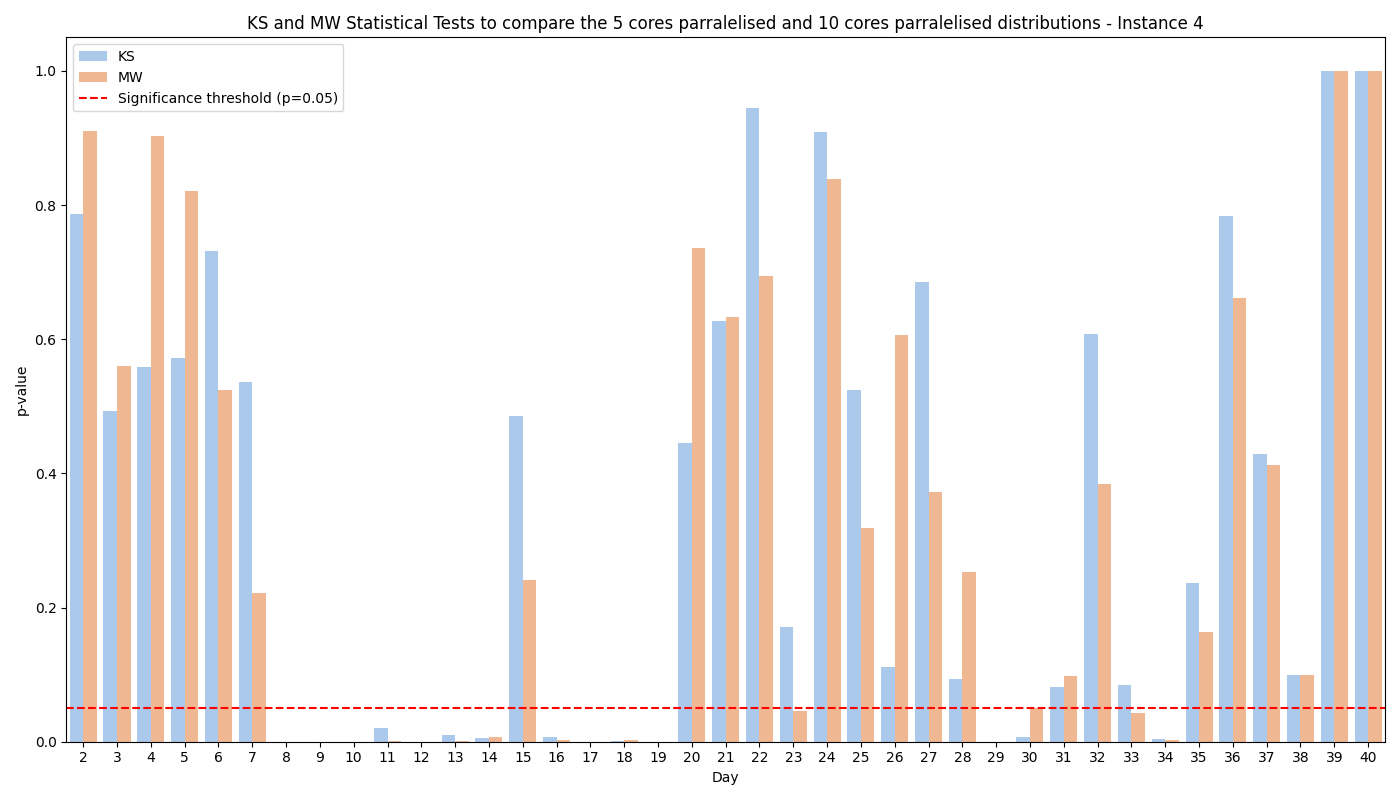
\includegraphics[width=.4\textwidth]{Figures/4 - Distribution stats tests 5P vs 10P.png}
    \caption{Statistical tests to compare the 5 \& 10 cores distribution - Instance 4}
    \label{fig:Stats test 5 VS 10 Parall}
\end{figure}


\section{Conclusion}

In this paper, a Monte Carlo Tree Search (MCTS) solution was implemented to address the Kiwi.com Travelling Salesman Problem 2.0, focusing on the first eight instances without imposing time constraints. The MCTS algorithm achieved solutions close to, or matching, the state-of-the-art solutions in several cases. Notably, for instance $I_8$, a new best solution was discovered, surpassing the previous best.

Regarding the selection policy, UCB1-Tuned outperformed the classic UCB by guiding the tree search more accurately through its consideration of simulation variability. However, UCB1-Tuned generally explores the tree more broadly and takes longer to converge compared to UCB. For expansion ratios, a lower ratio was preferred for smaller instances ($I_1, I_2, I_3$) to achieve faster solutions. Conversely, for other instances, a balanced ratio of 0.5 proved effective in incorporating new potential candidates into the solution space, thus accelerating the tree search. Nevertheless, the top-k expansion policy was superior, achieving solutions for $I_7$ and $I_8$ that were close to and better than the best-known solutions, respectively.

In terms of simulation policies, the greedy approach consistently provided the best performance across various instances, minimising the risk of the search becoming trapped in local optima due to the effectiveness of the selection policies. The tolerance policy, while offering a balanced approach, sometimes exhibited undesirable behaviour with more complex instances (e.g., $I_4$). The random policy, though effective for smaller instances, generally did not yield the best results and is therefore less favourable overall.

Finally, we recommend focusing on parallelisation within the MCTS framework. Parallelisation is especially beneficial when employing stochastic simulations, as it enhances the estimation of node values and improves the efficiency of the tree search. 

\bibliographystyle{IEEEtran}
\bibliography{Ref}

\end{document}
